\documentclass[12pt,a4paper]{article}

% Packages
% ---
\usepackage{amsmath}
\usepackage[utf8]{inputenc}
\usepackage[T1]{fontenc}
\usepackage[romanian]{babel}
\usepackage{graphicx}
\usepackage{listings}
\usepackage{setspace}
\usepackage{listings}
\usepackage[lmargin=2cm, rmargin=3cm]{geometry}
\usepackage{url}
\usepackage{xcolor}

\renewcommand{\lstlistingname}{Fragment de cod}

\lstset{language=C++, captionpos=b}

\graphicspath{ {./resources/} }

\fontfamily{Times New Roman}

\begin{document}

\onehalfspacing
\hyphenpenalty=10000
\exhyphenpenalty=10000

\begin{titlepage}
    \begin{center}
        \Large
        UNIVERSITATEA BUCUREȘTI
        \\FACULTATEA DE MATEMATICǍ ŞI INFORMATICǍ
        \\SPECIALIZAREA INFORMATICǍ
        \vspace*{0.5cm}
        \\
\includegraphics[width=4cm]{resources/blazon.png}

        \vspace*{2cm}
        \LARGE Lucrare de licență
        \\\huge Analiza statică a primitivelor de sincronizare
        
        \vfill
    \end{center}
    \large
    \hspace*{1.5cm}
    \begin{tabular}{c@{}}
        \textbf{Coordonator științific} \\
        \textbf{Paul Irofti}
    \end{tabular}
    \hfill
    \begin{tabular}{c@{}}
        \textbf{Absolvent} \\
        \textbf{Darius Marian}
    \end{tabular}
    \hspace*{1.5cm}
    \vspace*{1.5cm}
    \begin{center}
        \textbf{București, iulie 2020}
    \end{center}
\end{titlepage}

\newpage{} \tableofcontents{}

\newpage{}
\section{Introducere}
Programele cu mai multe fire de execuție au devenit mult mai comune
în programarea modernă. Procesoarele noi și plăcile grafice conțin mai
multe nuclee separate și capabilități de virtualizare, iar pentru a
folosi eficient aceste resurse, programele axate pe performanță
partajează sarcinile pe care le au de îndeplinit în mai multe fire de
execuție ce pot fi executate în paralel pe același hardware.

Dar prin introducerea acestui nou model de programare, s-a introdus și o
nouă gamă de dificultăți și posibilități de a face greșeli programatice.
Firele de execuție dintr-un proces accesează același spațiu de memorie
RAM, același disc, același monitor și alte dispozitive ale
calculatorului. De pildă dacă mai multe fire de execuție ce rulează
\textit{concurent} încearcă să stocheze informații diferite la aceeași
adresă de memorie RAM, rezultatul obținut nu este clar definit.
Problemele de acest tip se rezolvă folosind
\textit{mecanisme de sincronizare} pentru a controla și arbitra accesul
la resurse comune pe care mai multe fire de execuție le folosesc
concurent. Majoritatea acestor mecanisme sunt construite în jurul unor
\textit{primitive de sincronizare} printre care se numără
\textit{mutex}, \textit{semaphore}, \textit{read-write lock} și
\textit{condition variable}.

Folosirea acestor primitive este considerată dificilă. Orice resursă
partajată care este accesată concurent de mai multe fire de
execuție poate duce la un \textit{race condition} (o situație în care
rezultatul este nepredictibil pentru că depinde de ordinea în care
firele de execuție accesează resursa, dar de cele mai multe ori nu este
cel intenționat), așa că toate situațiile de acest tip din program
trebuie apărate folosind mecanisme de sincronizare. În același timp,
orice exces de astfel de mecanisme poate duce la alte tipuri de erori
cum ar fi \textit{deadlock} (situație în care două sau mai multe fire de
execuție se blochează reciproc, și niciuna nu mai poate progresa),
\textit{starvation} (un fir nu mai ajunge niciodată să își îndeplinească
sarcina pentru că nu mai primește acces la resursa partajată) sau
degradarea performanței programului (deoarece principalul motiv pentru
care se folosesc mai multe fire de execuție este performanța, aceasta
este de multe ori la fel de importantă ca și corectitudinea).

Dificultatea de înțelegere și utilizare a acestor concepte, împreună cu
rezultatele dezastruoase care apar frecvent din cauza erorilor de
programare crează o nevoie de unelte care să ajute dezvoltatorii de
aplicații în a identifica și repara acest tip de greșeli. Deși există
deja multe astfel de unelte în ecosistemul programării, nu toate
problemele ce pot apărea sunt rezolvate de unelte existente. De
asemenea, fiecare program care folosește aceste primitive de
sincronizare are alte nevoi, și o unealtă generică de multe ori nu poate
rezolva problemele specifice întâmpinate de un anumit program.

Vom prezenta în continuare un proiect ce are ca scop nu doar crearea
unei astfel de unelte, ci a unei platforme de dezvoltare ce facilitează
conceperea și implementarea de unelte noi și specifice unei anumite
nevoi printr-un efort minim.

\subsection{SyncAnalysis}
\textit{SyncAnalysis} este un proiect ce își propune crearea unui sistem
în care este ușor de dezvoltat unelte noi de diagnosticare a problemelor
ce pot apărea în folosirea mecanismelor primitive de sincronizare (și nu
doar).

Ideea din spatele acestui proiect vine din următoarea observație:
prin capturarea unor evenimente cheie pe parcursul execuției unui
program, se pot diagnostica o gamă largă de probleme pe care le
întâmpină acesta. Un exemplu simplu ar fi că prin observarea tuturor
cererilor de \textit{lock} și \textit{unlock} pe o instanță de
\textit{mutex}, se poate observa că \textit{mutex}-ul respectiv nu este
necesar dacă toate apelurile se întâmplă în contextul aceluiași fir de
execuție.

Din această observație se vede că proiectul folosește strategia
\textit{post-mortem} pentru analiza programelor: de-a lungul execuției
programului se înregistrează evenimentele de interes, pentru a fi
procesate și analizate separat după terminarea acestuia. Această
strategie a fost aleasă pentru că nu este deloc intrusivă: necesită
schimbări minime sau nule în codul sursă al programului (în anumite
situații nu necesită nici recompilarea codului sursă al unui
program) și nu degradează prea tare performanța programului în sine
pentru a face analiza. Alte strategii de analiză folosite în unelte
existente includ analiză \textit{on-the-fly}, în care analiza este
făcută în paralel cu execuția programului în același proces, precum în
ThreadSanitizer\cite{ThreadSanitizer} și analiză \textit{statică}, în
care codul sursă în sine este analizat, nu programul obținut prin
compilare, precum în Clang Thread Safety Analysis
\cite{ClangThreadSafetyAnalysis}.

Se distinge astfel direcția generală a acestui sistem. Prima și cea mai
importantă componentă este o bibliotecă ce înregistrează evenimentele
interesante în timpul execuției programului și le serializează într-un
fișier, pentru a fi analizate separat de alt program. Detalii despre
această bibliotecă și implementarea ei se găsesc în secțiunea
\textbf{\ref{library}}.

După execuția programului client obținem o colecție de evenimente,
capturate și serializate eficient într-un fișier cu ajutorul
bibliotecii descrise mai sus. În continuare, trebuie făcută o analiză
a acestor evenimente, iar proiectul oferă o soluție pentru asta în forma
unui program independent numit \lstinline{SyncAnalysis}. Acest program,
precum biblioteca de capturare a evenimentelor, este unul de uz general,
și nu este direct legat de analiza primitivelor de sincronizare. Acesta
nu execută pe cont propriu nicio analiză asupra evenimentelor, ci se
bazează pe o suită de module separate numite \textit{analizori}. Acești
analizori sunt distribuiți sub formă de biblioteci dinamice pe care
\lstinline{SyncAnalysis} le încarcă la începutul execuției. Programul se
ocupă de a deserializa și indexa evenimentele din fișier în memorie,
pentru ca apoi \textit{analizorii} să diagnosticheze erori, avertismente
sau în general informații utile pe baza acestor evenimente, iar
programul să creeze și să afișeze apoi rapoarte pentru utilizator. Mai
multe detalii despre acest program se găsesc în secțiunea
\textbf{\ref{executable}}, iar despre analizorii implementați ca exemplu
pentru analiza primitivelor de sincronizare în secțiunea
\textbf{\ref{analyzers}}.

Biblioteca și programul de analiză post-mortem sunt de uz general,
neavând în mod direct o interfață specifică analizării primitivelor de
sincronizare. De aceea proiectul conține și două exemple de biblioteci
pentru a facilita folosirea bibliotecii de capturare a evenimentelor în
scopul de analiză a primitivelor de sincronizare, descrise în detaliu în
Secțiunea \textbf{\ref{integration-libraries}}.

În Figura \ref{fig:architecture} se poate vedea arhitectura software a
proiectului SyncAnalysis. Cu albastru sunt marcate elementele de uz
general, adică cele independente de unealta dezvoltată (folosibile chiar
pentru unelte care nu se ocupă de analiza primitivelor de sincronizare),
cu verde sunt marcate elementele ce sunt specifice unei anumite unelte,
iar cu gri sunt marcate elementele programului client.

\begin{figure}[ht]
\centering
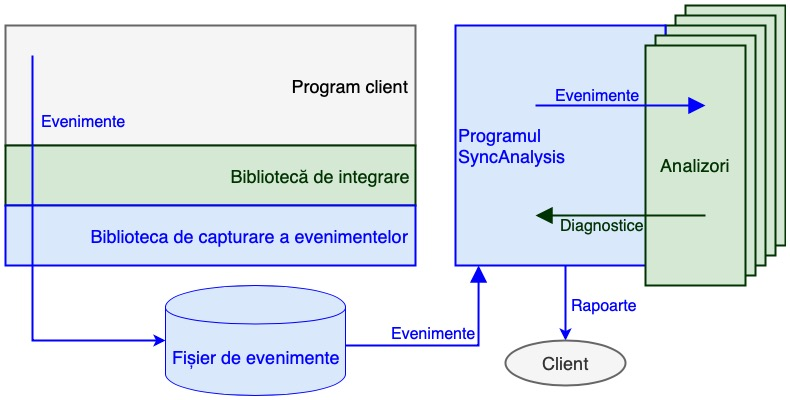
\includegraphics[width=14cm]{architecture.jpg}
\caption{Arhitectura proiectului SyncAnalysis}
\label{fig:architecture}
\end{figure}

\subsection{Comparație cu ThreadSanitizer}
O unealtă populară ce ajută la diagnosticarea folosirii insuficiente a
mecanismelor de sincronizare este ThreadSanitizer\cite{ThreadSanitizer}.
Folosirea acestuia implică compilarea programului cu un compilator care
implementează suport pentru ThreadSanitizer, folosind opțiunile de linie
de comandă documentate de compilator (de exemplu, pentru Clang pe Linux
opțiunea este \lstinline{-fsanitize=thread}). Executabilul obținut prin
compilare verifică toate scrierile în memoria RAM și emite erori dacă
o scriere este concurentă cu o alta sau cu o citire, și cele două nu
sunt explicit sincronizate.

\begin{lstlisting}[caption=Exemplu de folosire ThreadSanitizer]
% clang -fsanitize=thread -g -O1 -o program tiny_race.c
% ./program
WARNING: ThreadSanitizer: data race (pid=19219)
  Write of size 4 at 0x7fcf by thread T1:
    #0 Thread1 tiny_race.c:4 (exe+0xa360)
  Previous write of size 4 at 0x7fcf by main thread:
    #0 main tiny_race.c:10 (exe+0xa3b4)
  Thread T1 (running) created at:
    #0 pthread_create tsan_interceptors.cc:705 (exe+0xc790)
    #1 main tiny_race.c:9 (exe+0xa3a4)
\end{lstlisting}

După cum se vede din exemplul de mai sus (parafrazat din site-ul oficial
de documenție al proiectului \cite{ThreadSanitizerDoc}), ThreadSanitizer
analizează programul \textit{on-the-fly}: analiza este făcută direct în
cadrul execuției programului, în același proces. Asta duce la o
încetinire drastică a programului și la un consum ridicat de memorie.
Măsurătorile făcute pentru articolul \cite{ThreadSanitizer} arată o
creștere a timpului de execuție între 120\% și 2760\%, și în consumul de
memorie între 20\% și 660\%, în funcție de programul analizat. De
asemenea, ThreadSanitizer are nevoie de ajutor din partea
compilatorului, deci poate fi folosit doar cu compilatoare ce
încorporează explicit suport pentru el. Deși această unealtă este
folosită în companii mari din industrie \cite{ThreadSanitizer}, aceste
dezavantaje îl fac inutilizabil pentru anumite proiecte obligate să
folosească un anumit compilator care nu suportă ThreadSanitizer sau
care sunt executate în contexte unde reducerea drastică a performanței
nu este fezabilă nici măcar pentru teste sau simulări.

Prin comparație, o unealtă construită folosind proiectul SyncAnalysis
face analiza evenimentelor \textit{post-mortem}, și prin urmare nu duce
la creșteri atât de mari în consumul de timp sau memorie în timpul
execuției programului. În schimb fișierele de evenimente pot deveni
destul de mari dacă programul analizat este executat mult timp sau
capturează multe tipuri de evenimente.

\subsection{Comparație cu Clang-Tidy}
\textit{Clang-Tidy}\cite{ClangTidy} este o unealtă ce efectuează analiză
\textit{statică} asupra codului sursă a unui proiect. Deoarece analiza
se face static, fără a necesita execuția programului în sine,
considerentele de performanță a programului sunt inexistente: programul
compilat nu se schimbă din cauza folosirii uneltei, deci nu se aplică
problema de o degradare a performanței sau o creștere a resurselor
folosite din niciun punct de vedere.

Deși accentul nu este pus pe folosirea corectă sau eficientă a
primitivelor de sincronizare în cel din urmă, comparația dintre
proiectele \textit{SyncAnalysis} și \textit{Clang-Tidy} este aptă pentru
că amândouă încearcă să creeze un sistem de unelte, mai degrabă decât
să încerce să fie o unealtă de sine stătătoare. În timp ce proiectul
\textit{Clang-Tidy} permite scrierea cu efort mic a unor analizori
statici pentru codul sursă de C/C++, \textit{SyncAnalysis} face asta
pentru analizori \textit{post-mortem}.

\newpage{}
\section{Tehnologii folosite}

\subsection{Limbajul C11 și biblioteca standard C}

Limbajul C\cite{C} este folosit pentru implementarea bibliotecii de
înregistrare de evenimente și a uneia din bibliotecile de integrare.
Am ales limbajul pentru componenta aceasta din proiect deoarece
portabilitatea bibliotecii este o prioritate: această bibliotecă trebuie
să poată fi folosită în orice program scris în aproape orice limbaj și
rulând pe aproape orice sistem de operare. De asemenea este important ca
biblioteca să fie cât mai eficientă, pentru a nu interfera prea tare cu
execuția programului client. Această combinație de cerințe este
îndeplinită perfect de limbajul C. Am ales versiunea C11 pentru a avea
acces la modulul \lstinline{<stdatomic.h>} din biblioteca standard,
folosit în implementarea bibliotecii de înregistrare de evenimente din
motive de performanță.

\subsection{Limbajul C++17 și biblioteca standard C++}

Limbajul C++\cite{CXX} este folosit pentru implementarea majorității
proiectului. Programul \lstinline{SyncAnalysis}, una dintre bibliotecile
de integrare date ca exemplu, toate exemplele de analizoare și toate
testele automate au codul sursă scris în acest limbaj.

Înafară de preferință personală, argumentul principal pentru folosirea
limbajului C++ este interoperabilitatea bună cu limbajul C. Astfel, a
fost ușor de refolosit cod din biblioteca de înregistrare de evenimente
în programul SyncAnalysis pentru părțile de deserializare a fișierului
de evenimente, în timp ce restul programului și analizorii au putut fi
scriși într-un limbaj modern și foarte eficient. Biblioteca standard C++
este folosită peste tot în implementarea programului și în implementarea
analizorilor. Printre modulele folosite cel mai des se numără
\lstinline{<vector>}, \lstinline{<map>} și \lstinline{<string>}.

\subsection{Compilatorul Clang}

Limbajele C și C++, folosite în acest proiect, sunt limbaje a căror cod
sursă se compilează în cod nativ, executabil direct pe hardware. Pentru
a efectua această transformare în proiectul curent, am folosit exclusiv
compilatorul Clang\cite{Clang}, pentru portabilitatea acestuia între Mac
OS și Linux, viteza de compilare și integrarea elegantă cu alte unelte
de care am avut nevoie în dezvoltare cum ar fi
Clang-Tidy\cite{ClangTidy} și ThreadSanitizer\cite{ThreadSanitizer}.

\subsection{Uneltele de dezvoltare CMake și CTest}

Pentru proiecte mari de C++, invocarea manuală a compilatorului pentru
a recompila fiecare fișier modificat devine repede impractică.
CMake\cite{CMake} este un \textit{build system}: prin scrierea unui
fișier concis de configurare ce descrie structura fișierelor de cod
sursă din proiect, CMake automatizează recompilarea tuturor fișierelor
impactate de o schimbare, ducând astfel la o experiență plăcută de
dezvoltare a proiectului.

CTest este o componentă a proiectului CMake folosită pentru rularea
automată a testelor. Din nou, cu creșterea numărului de teste ce
trebuie efectuate după o schimbare în cod, devine impractică invocarea
manuală a acestora. CTest ajută la automatizarea acestui procedeu, din
nou spre a facilita o experiență plăcută de dezvoltare.

\subsection{Biblioteca pthread}

Biblioteca \lstinline{pthread}\cite{pthread} este interfața pentru
crearea și manipularea mai multor fire de execuție într-un proces. Este
parte din specificația standard POSIX pentru o interfață portabilă a
sistemelor de operare.

Biblioteca \lstinline{pthread} este folosită în ambele bibliotecile de
integrare, una din acestea având ca scop chiar simularea unei părți din
interfața publică oferită în antetul bibliotecii,
\lstinline{<pthread.h>}.

De asemenea, \lstinline{pthread} este folosită și în implementarea
bibliotecii de capturare de evenimente pentru crearea unui fir de
execuție separat care serializează evenimentele capturate în fișierul de
evenimente.

\subsection{Biblioteca DL}

Biblioteca \lstinline{DL}\cite{DL} este interfața descrisă în
specificația standard POSIX pentru găsirea, încărcarea și utilizarea
bibliotecilor dinamice. Această bibliotecă este folosită în proiect în
programul independent \lstinline{SyncAnalysis} pentru a încărca
analizorii specificați de client.

\subsection{Biblioteca libunwind}

Biblioteca \lstinline{libunwind}\cite{libunwind} este o facilitate
portabilă și eficientă pentru a observa stiva de apeluri de funcții în
timpul execuției unui program.

Biblioteca este folosită pentru a înregistra stiva de apeluri de funcții
când se capturează un eveniment. Folosirea bibliotecii acesteia este
preferabilă altor variante mai convenabile ce oferă direct simbolurile
asociate funcțiilor din stivă pentru că scopul bibliotecii de capturare
de evenimente este să fie cât mai eficientă, iar obținerea acestor
simboluri se poate face din programul \lstinline{SyncAnalysis}, după
terminarea programului client, doar pentru stivele de execuție necesare
în rapoarte.

\subsection{Programele addr2line, respectiv atos}

După cum s-a menționat și în secțiunea pentru \lstinline{libunwind},
biblioteca de capturare a evenimentelor serializează doar lista de
adrese din stiva de execuție în datele evenimentului în timpul execuției
programului client. Programul \lstinline{SyncAnalysis} transformă apoi
respectivele adrese în simboluri citibile de către client (nume de
funcții sau fișier și linie în codul sursă unde este făcut apelul),
pentru a fi atașate rapoartelor.

Pentru multe dintre sistemele de operare ce respectă standardul POSIX,
problema este rezolvată de programul \lstinline{addr2line} oferit de GNU
ca parte a proiectului \lstinline{binutils}\cite{binutils}. Programul
primește o listă de adrese de memorie ce reprezintă stiva de apeluri de
funcții și executabilul din care acestea au provenit și afișează exact
lista de simboluri asociate, și, dacă se pot afla, numele fișierului și
linia unde se află codul sursă pentru adresa respectivă din program.
Pentru că proiectul a fost dezvoltat în mare parte pe un calculator cu
sistemul de operare Mac OS (cu kernel-ul Darwin) unde programul
\lstinline{addr2line} nu dă rezultate satisfăcătoare, când se rulează
programul \lstinline{SyncAnalysis} pe Mac OS, acesta folosește
\lstinline{atos}\cite{atos} pentru a îndeplini aceleași sarcini.

\subsection{Biblioteca mcga-cli}

Programul \lstinline{SyncAnalysis} acceptă multe argumente de
configurare în linia de comandă (de exemplu directoarele în care să
caute analizori, reguli de includere și excludere pentru ce analizori
dintre cei găsiți să fie folosiți, dacă să afișeze sau nu informații
auxiliare pentru găsirea de erori în interiorul executabilului în sine
și altele).

Astfel, argumentele din linia de comandă sunt citite și interpretate
folosind o bibliotecă externă, \lstinline{mcga-cli}\cite{mcga-cli}.
Această bibliotecă a fost dezvoltată tot de autorul proiectului
\lstinline{SyncAnalysis} descris aici, dar este un proiect independent
de acesta.

\subsection{Git și GitHub}

Git\cite{git} este un sistem de versionare și menținere a istoricului de
modificări. A fost folosit în dezvoltarea acestui proiect exact cu acest
scop: de a menține un istoric central al tuturor modificărilor făcute
asupra codului sursă al proiectului și al acestui document.

GitHub\cite{GitHub} este o platformă comercială ce oferă un server de
git și o interfață web pentru a putea naviga ușor prin istoric.
\textit{Repository}-ul de git unde se găsește codul sursă al acestui
proiect este salvat pe serverul de git oferit de GitHub, și este
accesibil la adresa \url{https://github.com/darius98/sync-analysis}.

\newpage{}
\section{Descrierea proiectului}

\subsection{Instalarea și compilarea proiectului}
Proiectul poate fi descărcat, instalat și folosit pe orice calculator cu
sistemul de operare o distribuție de GNU/Linux sau Mac OS și cu acces
la internet. De asemenea, calculatorul trebuie să aibă instalate
următoarele programe:
\begin{itemize}
    \item \lstinline{as, ar, ld, addr2line} -- de obicei aceste programe
    sau alte programe echivalente vin preinstalate cu orice distribuție
    de GNU/Linux sau Mac OS. Ele fac parte din colecția de utilitare
    \lstinline{binutils}\cite{binutils} și sunt disponibile gratuit
    pentru descărcare pe website-ul oficial GNU\cite{GNUWebsite}.
    \item \lstinline{CMake}\cite{CMake} -- versiunea \lstinline{3.15}
    sau mai nouă
    \item \lstinline{make} -- orice versiune compatibilă cu versiunea de
    CMake instalată
    \item \lstinline{atos}\cite{atos} -- doar pentru Mac OS, unde este
    mereu preinstalat
    \item un compilator de C și C++ care suportă standardele C11,
    respectiv C++17 în întregime (de exemplu \lstinline{Clang 10}
    \cite{Clang})
    \item \lstinline{git}\cite{git} -- minim versiunea \lstinline{2.0}
\end{itemize}

Proiectul este disponibil pe internet, stocat pe server-ul GitHub.
Astfel, acesta poate fi descărcat prin următoarea comandă
\lstinline{shell}:

\begin{minipage}{\linewidth}
\begin{lstlisting}
    % git clone https://github.com/darius98/sync-analysis.git
\end{lstlisting}
\end{minipage}

Deoarece \textit{repository}-ul de git include biblioteca
\lstinline{mcga-cli}\cite{mcga-cli} ca submodul, trebuie executată o
comandă separată pentru a inițializa submodulele de git:

\begin{minipage}{\linewidth}
\begin{lstlisting}
    % cd sync-analysis/
    % git submodule update --init
\end{lstlisting}
\end{minipage}

Odată ce \textit{repository}-ul principal și \textit{submodul}-ul
\lstinline{mcga-cli} au fost descărcate cu succes, proiectul poate fi
compilat prin următoarea secvență de comenzi, executate în directorul de
bază al proiectului:

\begin{minipage}{\linewidth}
\begin{lstlisting}
    % cmake .
    % make all
\end{lstlisting}
\end{minipage}

După compilarea proiectului, acesta poate fi instalat în sistem folosind
următoarea comandă, executată tot în directorul de bază al proiectului:

\begin{minipage}{\linewidth}
\begin{lstlisting}
    % make install
\end{lstlisting}
\end{minipage}

Această comandă adaugă fișiere noi în directoarele de sistem. De obicei,
aceste fișiere se adaugă în directorul \lstinline{/usr/local/}, deci pe
multe sisteme această comandă va avea nevoie de permisiuni de
administrator. Soluția, de exemplu pe sistemul de operare Ubuntu, este
de a rula comanda folosind \lstinline{sudo}
(\lstinline{sudo make install}). Fișierele ce se adaugă în sistem prin
instalare sunt următoarele:

\begin{itemize}
    \item biblioteca pentru capturare de evenimente:
    \lstinline{lib/libsync_analysis.so} (pentru Mac OS extensia este
    \lstinline{.dylib}) și interfața C a acesteia:
    \lstinline{include/sync_analysis.h}
    \item biblioteca pentru integrare \lstinline{lib/libcxxsync.a} și
    interfața C++ a acesteia: directorul \lstinline{include/cxxsync/}
    \item biblioteca pentru integrare
    \lstinline{lib/libsyan_pthread_shim.so} (pentru Mac OS extensia este
    \lstinline{.dylib})
    \item biblioteca pentru integrare
    \lstinline{lib/libsyan_stdcxx_shim.so} (pentru Mac OS extensia
    este \lstinline{.dylib}) și interfața C++ a acesteia: directorul
    \lstinline{include/stdcxx_shim/}
    \item programul independent \lstinline{SyncAnalysis}
    \lstinline{bin/sync_analysis}
    \item interfața C++ pentru dezvoltarea analizorilor
    \lstinline{include/syan_analyzer_api/}
    \item analizorii preinstalați directorul \lstinline{syan-analyzers/}
\end{itemize}


\subsection{Biblioteca de capturare a evenimentelor}\label{library}
Aceasta este prima și cea mai importantă dintre componentele
proiectului. Pentru că această bibliotecă este încărcată direct în
programul clientului, este proiectată să fie atât portabilă cât și
performantă.

Pentru a maximiza portabilitatea, alegerea naturală de limbaj
pentru bibliotecă este C\cite{C}: pentru că limbajul are o interfață
binară standardizată de ISO și implementată de majoritatea
compilatoarelor folosite în industrie, împreună cu faptul că majoritatea
limbajelor de nivel înalt implementează
\textit{foreign-function-interface} cu C, aplicațiile pot beneficia de
această bibliotecă aproape indiferent de limbajul în care au fost
programate sau platforma pe care sunt executate.

Deși există variante mai bune pentru performanță cum ar fi C++ sau
\textit{assembly}, C este un limbaj suficient de eficient pentru a fi
cea mai bună alegere, luând în considerare avantajul copleșitor de
portabilitate.

\subsubsection{Interfață}\label{section:library-interface}
Pentru că această bibliotecă este una generică, interfața este
intenționat minimală: sunt expuse în mod public 3 funcții și 4
constante numerice. În limbajul C, interfața poate fi descrisă astfel:
\begin{lstlisting}[
        caption=Interfața bibliotecii pentru capturare de evenimente]
    void syan_capture_event(int event_type, void* object);

    void* syan_initialize_event(int event_type);
    void syan_finalize_event(void* event, void* object);

    enum {
      SA_EV_CREATE = 1 << 28,
      SA_EV_DESTROY = 1 << 29,
      SA_EV_THREAD = 1 << 30,
      SA_EV_THREAD_ON_CREATE = SA_EV_THREAD | SA_EV_CREATE,
    };
\end{lstlisting}
Această bibliotecă expune ca funcționalitate principală capturarea
evenimentelor, așa că interfața publică importantă este funcția
\lstinline{syan_capture_event}, care îndeplinește exact acest scop.
Toate celelalte componente ale interfeței expuse sunt pentru a trata
cazuri particulare mai complexe sau a standardiza tipuri de evenimente
pe care se bazează și programul \lstinline{SyncAnalysis}, și sunt
descrise mai jos. Exemplul principal de utilizare după care a fost
proiectată funcția \lstinline{syan_capture_event} se poate vedea în
Fragmentul de cod \ref{code:library-interface-example}.

\begin{lstlisting}[caption=Exemplul folosit în proiectarea interfeței,
                   label=code:library-interface-example]

    #define EVENT_MUTEX_BEFORE_LOCK 1331
    #define EVENT_MUTEX_AFTER_LOCK 1332

    pthread_mutex_t* m;
    void f() {
        syan_capture_event(EVENT_MUTEX_BEFORE_LOCK, m);
        pthread_mutex_lock(m);
        syan_capture_event(EVENT_MUTEX_AFTER_LOCK, m);
    }
\end{lstlisting}

Funcția este apelată cu 2 parametri, unul pentru tipul de eveniment
capturat și celălalt pentru identitatea obiectului țintă al
evenimentului. Astfel, în analiza post-mortem a unui program se poate
face o corelare între mai multe evenimente care au avut loc pe același
obiect țintă. Cum obiectele în limbajul C au în mod implicit o
identitate dată de adresa de memorie unde sunt stocate, este natural ca
parametrul care identifică obiectul să aibă tipul de date
\lstinline{void*}, care reprezintă în mod convențional o adresă oarecare
de memorie. Apare totuși o problemă: aceași adresă de memorie poate fi
refolosită de-a lungul execuției unui program, pentru a stoca mai multe
obiecte logice diferite (după dealocarea primului obiect, la alocarea
unui obiect nou se poate folosi aceași memorie; un exemplu comun este
segmentul de memorie stivă al programului). Pentru a evita confuzii
generate de această problemă, biblioteca expune două constante numerice
\lstinline{SA_EV_CREATE} și \lstinline{SA_EV_DESTROY}, ce acționează ca
\textit{biți indicatori} în tipul unui eveniment: dacă în scrierea în
baza 2 a tipului unui eveniment bitul \lstinline{SA_EV_CREATE}
(respectiv \lstinline{SA_EV_DESTROY}) este 1, evenimentul este
considerat unul care marchează crearea un obiect (respectiv distrugerea
unui obiect).

Această convenție este folosită și de către programul
\lstinline{SyncAnalysis}, care se folosește de aceste evenimente pentru
a reconstrui o bază de date de obiecte active în fiecare punct al
execuției programului client, a include evenimentul ce marchează
crearea unui obiect țintă în rapoarte și a elibera memorie după
distrugerea unui obiect. Astfel, este recomandat ca orice bibliotecă de
integrare să folosească acești indicatori pentru a captura evenimente ce
marchează crearea și distrugerea tuturor obiectelor de interes pentru
evenimentele capturate de respectiva bibliotecă:
\begin{lstlisting}
    enum {
        EVENT_MUTEX = 1u << 15,
        EVENT_MUTEX_CREATE = EVENT_MUTEX | SA_EV_CREATE,
        EVENT_MUTEX_DESTROY = EVENT_MUTEX | SA_EV_DESTROY,
    };
\end{lstlisting}

Fiecare eveniment capturat conține identitatea firului de execuție care
l-a capturat. Este util atunci să se raporteze câte un eveniment care
marchează crearea fiecărui fir de execuție, pentru a putea pune
evenimentele capturate de un anumit fir de execuție într-un context.
Astfel, biblioteca în sine când se încarcă capturează ca prim eveniment
unul care marchează crearea firului de execuție care a încărcat
biblioteca. Pentru că biblioteca raportează în interiorul său un
eveniment de creare de fir de execuție, aceasta stabilește un număr
\lstinline{SA_EV_THREAD_ON_CREATE} (se observă în interfață că acest
număr conține bitul \lstinline{SA_EV_CREATE}) care să reprezinte
evenimentele de acest tip. Orice bibliotecă de integrare trebuie să dea
același număr pentru argumentul \lstinline{event_type} când apelează
funcția \lstinline{syan_capture_event} pentru a raporta crearea unui fir
nou de execuție.

Cu experiența implementării bibliotecilor de integrare s-a observat că
atunci când se raportează crearea unui nou fir de execuție folosind
biblioteca \lstinline{pthread}, identitatea obiectului țintă
al evenimentului este cunoscută abia după ce a pornit noul fir de
execuție:
\begin{lstlisting}[caption=Capturare incorectă a creării unui fir de
                           execuție]
    pthread_t T;
    pthread_create(&T, nullptr, func, arg);
    syan_capture_event(SA_EV_THREAD_ON_CREATE, (void*)T);
\end{lstlisting}
Dacă evenimentul care marchează crearea firului de execuție \textit{T}
este capturat \textit{după} crearea lui \textit{T}, pot apărea
inconsistențe în analiza post-mortem: firul de execuție \textit{T} poate
începe să captureze evenimente, care pot ajunge să apară în fișierul de
evenimente înaintea evenimentului care marchează crearea lui \textit{T}.
Pentru a rezolva această situație, biblioteca expune celelalte două
funcții \lstinline{syan_initialize_event} și
\lstinline{syan_finalize_event} în interfața bibliotecii.  Funcția
\lstinline{syan_initialize_event} crează evenimentul și îi alocă locul
în fișierul de evenimente \textit{înainte} de crearea firului
\textit{T}. După crearea firului \textit{T}, evenimentul este doar
marcat ca fiind \textit{finalizat}, dar este scris în fișier ca și cum
în locul unde a fost mai înainte apelat
\lstinline{syan_initialize_event} ar fi fost apelat
\lstinline{syan_capture_event}, rezolvând problema ridicată mai devreme.
Exemplul de mai sus se repară astfel:
\begin{lstlisting}[caption=Capturare corectă a creerii unui fir de
                           execuție]
    pthread_t T;
    void* ev = syan_initialize_event(SA_EV_THREAD_ON_CREATE);
    pthread_create(&T, nullptr, func, arg);
    syan_finalize_event(ev, (void*)T);
\end{lstlisting}

Se observă acum că funcția \lstinline{syan_capture_event} are o
implementare evidentă pe baza celor două funcții nou introduse:
\begin{lstlisting}[caption=Implementarea funcției
                   \lstinline{syan_capture_event}]
    void syan_capture_event(int event_type, void* object) {
        void* ev = syan_initialize_event(event_type);
        syan_finalize_event(ev, object);
    }
\end{lstlisting}

\subsubsection{Structura unui eveniment}\label{section:event-structure}

Un eveniment capturat de bibliotecă are aceași structură indiferent de
tipul evenimentului sau de identitatea obiectului țintă al acestuia.
Aceasta a fost proiectată astfel încât mai multe evenimente să poată fi
stocate ușor și eficient într-o zonă continuă de memorie și serializate
în format binar pe disc. În codul sursă C al bibliotecii, structura ce
definește un eveniment se poate vedea în Fragmentul de cod
\ref{code:event-structure}.
\begin{lstlisting}[caption=Structura unui eveniment capturat,
                   label=code:event-structure, float, floatplacement=H]
    typedef struct {
        int32_t signature;
        int32_t event_type;
        int64_t timestamp;
        intptr_t thread_id;
        intptr_t object_id;
        intptr_t backtrace[12];
    } SyanEvent;
\end{lstlisting}

Ordinea și dimensiunea în biți a fiecărui câmp a fost aleasă astfel
încât pe platformele cele mai populare, unde arhitectura procesorului
este pe 64 de biți și astfel dimensiunea unui \lstinline{intptr_t} este
8 bytes, un eveniment să aibă dimensiunea exact 128 bytes, fără spațiu
irosit din cauze precum \textit{padding} sau \textit{alignment}. Această
dimensiune, fiind o putere a lui 2 ($2^7=128$) mai are un avantaj:
dimensiunea paginii de RAM este în general tot o putere de 2, de obicei
4096 ($2^{12}$), și astfel pe o pagină de memorie încap exact 32 de
evenimente. Această proprietate este exploatată în bibliotecă pentru a
obține viteze mari de serializare a evenimentelor în memorie, și mai
apoi pe disc.

Câmpul \lstinline{signature} este folosit intern pentru a împiedica
biblioteca din a scrie un eveniment pe disc înainte de apelarea funcției
\lstinline{syan_finalize_event} pentru acel eveniment. Aceasta nu va
scrie evenimentul pe disc până când nu citește în câmpul
\lstinline{signature} valoarea prestabilită 666013. Valoarea câmpului
este 0 după apelul la funcția \lstinline{syan_initialize_event}, dar
evenimentul este deja pus în coada de evenimente ce trebuie scrise pe
disc. Când este apelată funcția \lstinline{syan_finalize_event},
valoarea este schimbată în 666013, permițând bibliotecii să continue
scrierea evenimentelor din coadă pe disc.

Câmpurile \lstinline{event_type} și \lstinline{object_id} vor conține
valorile date ca parametri de către client când acesta apelează funcția
\lstinline{syan_capture_event}, sau respectiv funcțiile
\lstinline{syan_initialize_event} și \lstinline{syan_finalize_event}.

Câmpul \lstinline{timestamp} este o reprezentare pe 64 de biți al
numărului de nanosecunde scurse de la inițializarea bibliotecii până la
momentul capturării evenimentului. Fișierul DUMP (descris în secțiunea
\textbf{\ref{dump-file}}) conține în \textit{header} momentul de timp al
inițializării bibliotecii, astfel momentul real de timp când a avut loc
evenimentul poate fi reconstruit post-mortem cu precizie de nanosecundă,
iar stocarea numărului de nanosecunde pe 64 de biți permite capturarea
evenimentelor într-un program cu durată de viață până la 146 de ani,
suficient pentru orice scop practic.

Câmpul \lstinline{thread_id} conține identitatea firului de execuție ce
a capturat evenimentul. Acesta este obținut printr-un apel la funcția
\lstinline{pthread_self()}, descrisă în specificația POSIX pentru fire
de execuție portabile\cite{pthread}. Deși specificația nu precizează
dacă tipul de date returnat de \lstinline{pthread_self()}, anume
\lstinline{pthread_t}, poate fi stocat cu succes într-o variabilă cu
tipul de date \lstinline{intptr_t}, în practică toate implementările
bibliotecii \lstinline{pthread} pentru platformele pe care a fost
testată biblioteca implementează \lstinline{pthread_t} ca pe un
\textit{pointer} la structura de control a firului de execuție (iar
acest \textit{pointer} poate fi stocat, conform definiției tipului de
date \lstinline{intptr_t}).

Câmpul \lstinline{backtrace} conține adresele de întoarcere din stiva de
execuție. Acestea sunt utile pentru ca în analiza post mortem să se
poată reconstrui stiva de apeluri de funcții așa cum este descris în
secțiunea \textbf{\ref{stack-reconstruction}} și să se poată construi
rapoarte cât mai exacte despre condițiile în care s-a capturat un
eveniment. Modul cum sunt capturate aceste adrese este descris mai pe
larg în secțiunea \textbf{\ref{stack-unwinding}}.

\subsubsection{Stiva de execuție}\label{stack-unwinding}

După compilarea programelor în cod de asamblare, tot codul este
structurat în funcții. Când o funcție apelează o altă funcție, aceasta
trebuie să își stocheze valorile variabilelor locale în memorie și
trebuie să îi transmită funcției apelate adresa de memorie unde să
reîntoarcă controlul odată ce și-a terminat execuția. Zona de memorie
unde funcțiile stochează aceste informații se numește segmentul de stivă
al programului. Fiecare fir de execuție are propriul segment stivă,
independent de celelalte fire.

\begin{figure}[ht]
\centering
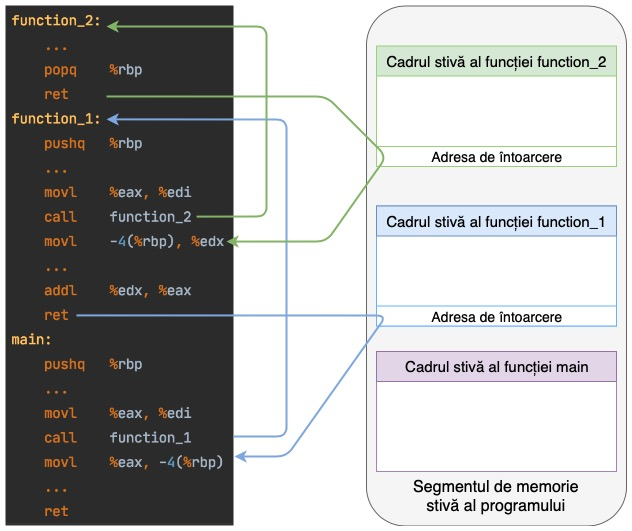
\includegraphics[width=14cm]{stack.jpg}
\caption{Stiva de execuție în arhitectura X86}
\label{fig:stack}
\end{figure}

În Figura \ref{fig:stack} se poate vedea acest procedeu pentru
arhitectura X86: în momentul apelului funcției \lstinline{function_1}
din funcția \lstinline{main}, se crează un nou cadru în memoria stivă a
programului (identificată pe desen prin culoarea albastru). La începutul
acestui cadru se stochează adresa de memorie a instrucțiunii următoare
apelului din funcția \lstinline{main}. În timpul execuției funcției
\lstinline{function_1}, aceasta apelează o a doua funcție
\lstinline{function_2}. Se crează deci un al treilea cadru în memoria
stivă (identificată pe desen prin culoarea verde), din nou stocându-se
adresa de întoarcere. La finalul funcției \lstinline{function_2},
aceasta invocă instrucțiunea \lstinline{ret}, care întoarce controlul la
adresa de memorie stocată în cadrul de stivă al funcției curente, adică
înapoi la funcția \lstinline{function_1}. Când și aceasta se termină
prin invocarea instrucțiunii ret, controlul este întors funcției
\lstinline{main}. Dacă aceasta nu mai este apelată la rândul său de
nicio altă funcție, instrucțiunea \lstinline{ret} de la sfârșitul
acesteia va încheia execuția programului, întorcând controlul sistemului
de operare.

A se observa că explicația dată mai sus nu descrie în mod exact cum
funcționează procesoarele și programele moderne, însă putem ajunge la
rezultate corecte pentru scopul nostru și fără a înțelege alte detalii
sau complicații istorice ale stivei de execuție. Singurul detaliu demn
de menționat este că în unele situații, compilatoarele de C și C++ pot
decide să \textit{optimizeze} programul prin omiterea stocării adresei
de întoarcere pe stivă, caz în care reconstruirea stivei de execuție
devine imposibilă. Pentru compilatorul Clang\cite{Clang}, această
optimizare poate fi oprită prin argumentul de compilare
\lstinline{-fno-omit-frame-pointer}.

Dacă funcția \lstinline{function_2} face un apel la funcția
\lstinline{syan_capture_event} pentru a captura un eveniment, vrem să
obținem lista de adrese de întoarcere din toate cadrele funcțiilor din
stivă. Acest rezultat poate fi obținut folosind biblioteca
\textit{libunwind}\cite{libunwind}, după cum se poate vedea în
Fragmentul de cod \ref{code:stack-unwinding}.

\begin{lstlisting}[caption=Capturarea stivei de execuție folosind
                           \lstinline{libunwind},
                   label=code:stack-unwinding,
                   float, floatplacement=H]
    #include <libunwind.h>
    void syan_get_backtrace(intptr_t* backtrace) {
        unw_context_t ctx;
        unw_getcontext(&ctx);
        unw_cursor_t crs;
        unw_init_local(&crs, &ctx);
        int n_frames = 0;
        while (n_frames < 12 && unw_step(&crs) > 0) {
            unw_word_t ip;
            if (unw_get_reg(&crs, UNW_REG_IP, &ip) < 0) break;
            backtrace[n_frames++] = (intptr_t)ip;
        }
    }
\end{lstlisting}

\subsubsection{Coada de evenimente și serializarea}\label{section:queue}

Am menționat deja mai devreme că un obiectiv în proiectarea acestei
biblioteci este ca performanța programului analizat să fie impactată cât
se poate de puțin. Trebuie luat în considerare astfel că scrierea
evenimentelor pe disc este o operațiune lentă. Prima decizie luată în
implementarea serializării este deci de a scrie evenimentele doar în
memoria RAM în cadrul firelor de execuție ale programului client, pentru
ca mai apoi un alt fir de execuție creat de bibliotecă să copieze datele
din memoria RAM pe disc. Pentru a obține rezultate satisfăcătoare de
performanță, am proiectat o \textit{coadă de evenimente} (intern numită
\lstinline{SyanBuffer}) specifică pentru această bibliotecă. Interfața
acestei cozi se poate vedea în Fragmentul de cod
\ref{code:queue-interface}.

\begin{lstlisting}[caption=Interfața cozii de evenimente folosite în
                           bibliotecă,
                   label=code:queue-interface, float, floatplacement=H]
#define SYAN_BUFFER_PAGE_SIZE 256
#define SYAN_BUFFER_NUM_PAGES 1024
typedef struct {
    SyanEvent storage[SYAN_BUFFER_PAGE_SIZE];
    int_fast32_t storage_front;
    atomic_int_fast32_t storage_back;
} SyanBufferPage;
typedef SyanBufferPage* SyanBufferPagePtr;
typedef struct {
    SyanBufferPagePtr pages[SYAN_BUFFER_NUM_PAGES];
    int_fast32_t pages_front;
    atomic_int_fast32_t pages_back;
} SyanBuffer;
int syan_buffer_init(SyanBuffer** b);
SyanEvent* syan_buffer_acquire_event_slot(SyanBuffer* b);
SyanBufferPagePtr syan_buffer_get_front_page(SyanBuffer* b);
void syan_buffer_release_front_page(SyanBuffer* b);
\end{lstlisting}
Prima proprietate importantă a acestei cozi este că nu conține niciun
mecanism explicit de sincronizare, ci doar câteva variabile cu tipul de
date \textit{atomic}. Minimizarea latenței punerii evenimentelor în
coadă este mai importantă decât eficiența citirii din coadă, pentru a
interfera cât mai puțin cu firele de execuție ale programului client.
Când un astfel de fir capturează un eveniment, memoria folosită pentru
a stoca informațiile acelui eveniment este direct memorie din câmpul
\lstinline{storage} al paginii curente din coadă (mai exact pagina
\lstinline{b->pages[b->pages_back]}). Asta omite necesitatea de a apela
funcții precum \lstinline{malloc} pentru a obține memorie pentru fiecare
eveniment individual sau \lstinline{memcpy} pentru a muta evenimentul
în coadă abia după ce acesta este complet format. Așadar funcția
\lstinline{syan_initialize_event} obține memoria necesară pentru
stocarea evenimentului apelând funcția
\lstinline{syan_buffer_acquire_event_slot}. Aceasta este implementată
folosind un algoritm \textit{lock-free} bazat pe operațiile de
\textit{compare-and-swap} și \textit{atomic-fetch-add} pe variabilele
atomice \lstinline{pages_back} și respectiv \lstinline{storage_back} din
acea pagină. Implementarea este similară cu cele descrise în articolele
\textit{Lock-free linked lists using compare-and-swap}
\cite{LinkedListsCAS} și
\textit{A practical nonblocking queue algorithm using compare-and-swap}
\cite{QueueCAS}.

După ce un eveniment a fost scris în coadă, acesta trebuie scris mai
departe pe disc. După cum am spus mai sus, biblioteca crează un fir de
execuție special pentru această operație. Fiind un singur fir care se
ocupă de scrierea pe disc a evenimentelor de la începutul cozii, se
poate observa și în interfață că variabilele \lstinline{pages_front} și
\lstinline{storage_front} nu sunt atomice: aceasta sunt atât scrise cât
și citite doar de firul intern al bibliotecii, așa că nu necesită
sincronizare. Am menționat și mai devreme cum un eveniment pus în coadă
nu este scris pe disc până când câmpul \lstinline{signature} al
evenimentului nu are valoarea corectă, scrisă de apelul funcției
\lstinline{syan_finalize_event}. În practică, firul de execuție al
bibliotecii citește aceste semnături din evenimentele de la începutul
cozii folosind operația \textit{atomic-load}, pentru că se așteaptă ca
scrierea să fie făcută de firul de execuție care raportează evenimentul.

Firul de execuție intern bibliotecii funcționează pe bază de iterații:
o iterație scrie cât de multe evenimente poate din coadă pe disc. Dacă
iterația a scris cu succes date pe disc, se trece direct la următoarea
iterație. Altfel, înseamnă că nu mai există evenimente noi capturate, și
firul apelează funcția de sistem \lstinline{usleep} pentru a permite
firelor programului client să își continue execuția înainte de a începe
o nouă iterație. Pentru a afla ce evenimente noi trebuie scrise pe disc,
firul verifică valorile câmpurilor \lstinline{storage_front} și
\lstinline{storage_back} de pe cea mai veche pagină a cozii, obținută
printr-un apel la funcția \lstinline{syan_buffer_get_front_page}. Dacă
valorile acestea sunt diferite, atunci toate evenimentele dintre sunt
fie evenimente noi capturate, fie evenimente în curs de capturare. Firul
așteaptă finalizarea tuturor acestor evenimente pe modelul
\textit{busy-wait}, deoarece se asumă că apelurile funcțiilor
\lstinline{syan_initialize_event} și \lstinline{syan_finalize_event}
se fac la puțin timp unul după celălalt. S-a experimentat aici și cu
alte modele de așteptare (\lstinline{pthread_sched_yield},
\lstinline{usleep}) și s-a observat empiric că \textit{busy-wait} se
comportă cel mai bine în practică. După ce toate aceste evenimente sunt
finalizate, ele sunt scrise împreună pe disc printr-un singur apel al
funcției standard C \lstinline{fwrite}. Dacă prin scrierea acestor
evenimente s-au scris toate evenimentele din pagină, aceasta este
eliberată. Altfel, se modifică doar câmpul \lstinline{storage_front} al
paginii pentru a marca până unde au fost scrise evenimentele din pagină.

\subsubsection{Fișiserului DUMP}\label{dump-file}

Am menționat în repetate rânduri că evenimentele capturate în timpul
execuției sunt scrise într-un fișier, denumit în continuare fișierul
DUMP. Dar acest fișier nu conține doar evenimentele, ci are și un antet
ce conține informații în plus despre execuție, utile pentru analiza
post-mortem a evenimentelor:
\begin{itemize}
    \item momentul când a fost inițializată biblioteca (o aproximare
    bună a momentului când a început execuția programului)
    \item calea către executabilul invocat
    \item argumentele din linia de comandă date executabilului
    \item adresa la care a fost încărcat executabilul
\end{itemize}

Momentul când a fost inițializată biblioteca este important pentru a
putea reconstrui momentul de timp când a fost capturat un eveniment,
pentru că valoarea câmpului \lstinline{timestamp} din fiecare eveniment
este egală cu numărul de nanosecunde ce au trecut între acest moment de
inițializare și momentul capturării evenimentului.

Calea către executabiul invocat și argumentelee din linia de comandă
sunt utile pentru a putea identifica ce reprezintă acest fișier DUMP. Nu
sunt folosite de către programul \lstinline{SyncAnalysis} decât pentru a
fi afișate în raportul de analizare.

Adresa de încărcare a executabilului este importantă pentru a putea
interpreta adresele din \lstinline{backtrace}-urile evenimentelor. Mai
multe detalii despre acest procedeu se găsesc în secțiunea 
\textbf{\ref{stack-reconstruction}}.

Fișierul DUMP este creat și deschis pentru scriere printr-un apel la
funcția standard C \lstinline{fopen("sync_analysis.dump", "wb")}.
Conform specificației acestei funcții, dacă un fișier cu același nume
exista deja, versiunea anterioară este ștearsă și un nou fișier gol este
creat oricum. Apelul la \lstinline{fopen} se face la inițializarea
bibliotecii, împreună cu scrierea antetului și pornirea firului intern
de execuție. În continuarea antetului sunt scrise direct evenimentele,
unul după celălalt, serializate în formatul binar descris în secțiunea
\textbf{\ref{section:event-structure}}.

\subsubsection{Măsurători de performanță}\label{library-performance}

Performanța bibliotecii se împarte în două metrici diferite: timpul
necesar capturării unui eveniment (metrica de \textit{latență}) și
volumul de evenimente ce poate fi serializat într-o perioadă de timp
(metrica de \textit{debit}). În Figurile \ref{fig:lib-perf-latency} și
\ref{fig:lib-perf-throughput} se pot vedea tabel cu măsurătorile
efectuate cu ajutorul bibliotecii
\lstinline{Google Benchmark}\cite{GoogleBenchmark} pentru ambele
metrici.

\begin{figure}[H]
\centering

\begin{center}
    \begin{tabular}{||c c||} 
        \hline
        Numărul firelor de execuție & Latența capturării unui eveniment \\ [0.5ex] 
        \hline\hline
        1 & 569 ns \\ \hline
        2 & 601 ns \\ \hline
        3 & 615 ns \\ \hline
        4 & 670 ns \\ \hline
        5 & 811 ns \\ \hline
        6 & 1080 ns \\ \hline
    \end{tabular}
\end{center}

\caption{Măsurători de latență a bibliotecii}
\label{fig:lib-perf-latency}
\end{figure}

\begin{figure}[H]
\centering

\begin{center}
    \begin{tabular}{||c||} 
        \hline
        Debitul maxim pentru serializarea pe disc a evenimentelor \\ [0.5ex] 
        \hline\hline
        5'190'780 evenimente/secundă \\ \hline
    \end{tabular}
\end{center}

\caption{Măsurători de debit al bibliotecii}
\label{fig:lib-perf-throughput}
\end{figure}

Metrica de \textit{latență} este măsurată în \textit{nanosecunde} (cât
timp durează capturarea unui eveniment) și depinde de numărul de fire de
execuție ce capturează evenimente concurent, pentru că operațiile
\textit{compare-and-swap} implicate în acest procedeu au șansă mai mare
să eșueze cu cât sunt mai multe fire care încearcă să le execute în
același timp.

Metrica de \textit{debit} este măsurată în \textit{evenimente/secundă}
(câte evenimente pot fi serializate pe disc într-o perioadă de timp) și
nu depinde de nimic: aceasta reprezintă numărul \textit{maxim} de
evenimente a căror serializare poate fi cerută până când biblioteca nu
mai poate serializa evenimentele la viteza cu care vin acestea.


\subsection{Biblioteci de integrare}
\label{integration-libraries}

\subsubsection{Interfața pentru primitive de sincronizare}

Biblioteca pentru capturare de evenimente este una generică, ce nu oferă
o interfață specială pentru evenimente specifice primitivelor de
sincronizare. Pentru a construi câteva exemple de analizori pentru
primitive de sincronizare, am proiectat o interfață simplă ce conține
o enumerație a evenimentelor 

\subsubsection{cxxsync (C++, începând cu C++98)}

\subsubsection{pthread shim (C/C++)}

\subsubsection{libc++ shim (pentru C++, începând cu C++11)}


\subsection{Programul independent SyncAnalysis}
\label{executable}

\subsubsection{Parcurgerea și parsarea fișierului DUMP}

\subsubsection{Stocarea și observarea obiectelor active}

\subsubsection{Crearea de rapoarte}

\subsubsection{Afișarea simbolurilor din stiva de execuție}
\label{stack-reconstruction}

\subsubsection{Înregistrarea analizorilor}


\subsection{Analizori pre-instalați}
\label{analyzers}

\subsubsection{mutex-lock-order}

\subsubsection{lock-shadow}

\subsubsection{redundant-recursive-mutex}

\subsubsection{redundant-rwlock}

\subsubsection{useless-lock}


\newpage{}
\section{Exemple de utilizare}
\subsection{Testele analizorilor (folosind cxxsync)}
\subsection{Folosind LD\_PRELOAD și <pthread.h>}
\subsection{Folosind libc++}

\newpage{}
\section{Concluzii}

\todo{Write text}

\newpage{}

\appendix
\renewcommand{\listfigurename}{Anexa A. Lista figurilor}
\listoffigures
\renewcommand{\lstlistlistingname}{Anexa B. Lista fragmentelor de cod}
\lstlistoflistings

\bibliographystyle{unsrt}
\bibliography{bibliografie}

\end{document}
